\Chapter{RÉSULTAT}\label{sec:Theme2}

Les résultats sont présentés en commençant d’abord par décrire l’implémentation du modèle conceptuel d’automate présenté dans la sous-section~\ref{subsection_cadre_conceptuel}. Ensuite, ce sera présenté successivement les résultats propres à chacun des sous-objectifs décrits dans le chapitre~\ref{chapitre_methode}.

\section{Implémentation: du modèle conceptuel au modèle opérationnel}

L’implémentation de la machine (conceptuelle) est passée par la programmation manuelle d’une première interface et d’un premier noyau, en mettant à jour une version préliminaire de générateur basé sur une GUI\cite{bluiksnot_repo} en lui intégrant la capacité de générer du code à partir d’un module externe via son «hook» au moment de l’installation. La version à ce jour, ainsi que ses guides d’utilisation et ses scripts associés, sont disponibles sur le site de ERPLibre\footnote{\url{https://erplibre.ca}}.

L’interface permet l’interactivité avec un utilisateur ou le système-cible. L’interface est découplée en deux ensembles de méta-données: µ$_C^A$ et µ$_C^B$. µ$_C^B$ est l’ensemble qui paramétrise le passage de méta-données au code pour un module spécifique. µ$_C^A$ est l’ensemble qui paramétrise le passage de code aux méta-données tout en préparant un µ$_C^B$ adapté à ce module spécifique. Ce découplage a permis l’adaptation de l’interface au contexte de l’installation de modules sur une instance Odoo via des «hooks». Par la suite, un ensemble supplémentaire de méta-données, noté µ$_C^0$, a été dégagé de la programmation manuelle de versions successives de µ$_C^A$. µ$_C^0$ sert à initialiser une version de départ de µ$_C^A$.

Le noyau prend les paramètres issus de l’interface pour créer des méta-données, générer l’ensemble des fichiers des modules désirés (mode direct) et faire de la rétro-ingénierie (mode indirect) sur des modules existants.

\subsection{Développement et amélioration continue}

Dans la figure~\ref{fig:dia_sequence_gc}, µ$_C^0$, µ$_C^A$, µ$_C^B$, C et M sont tous des modules installables sur Odoo. $M^i$ et $M^d$ sont des sections de code dans le module M. µ$_C^0$, µ$_C^A$ et µ$_C^B$ dépendent de M. µ$_C^A$, c’est les macro-méta-données, que µ$_C^B$, c’est les micro-méta-données.

\begin{figure}[htb]
\centering
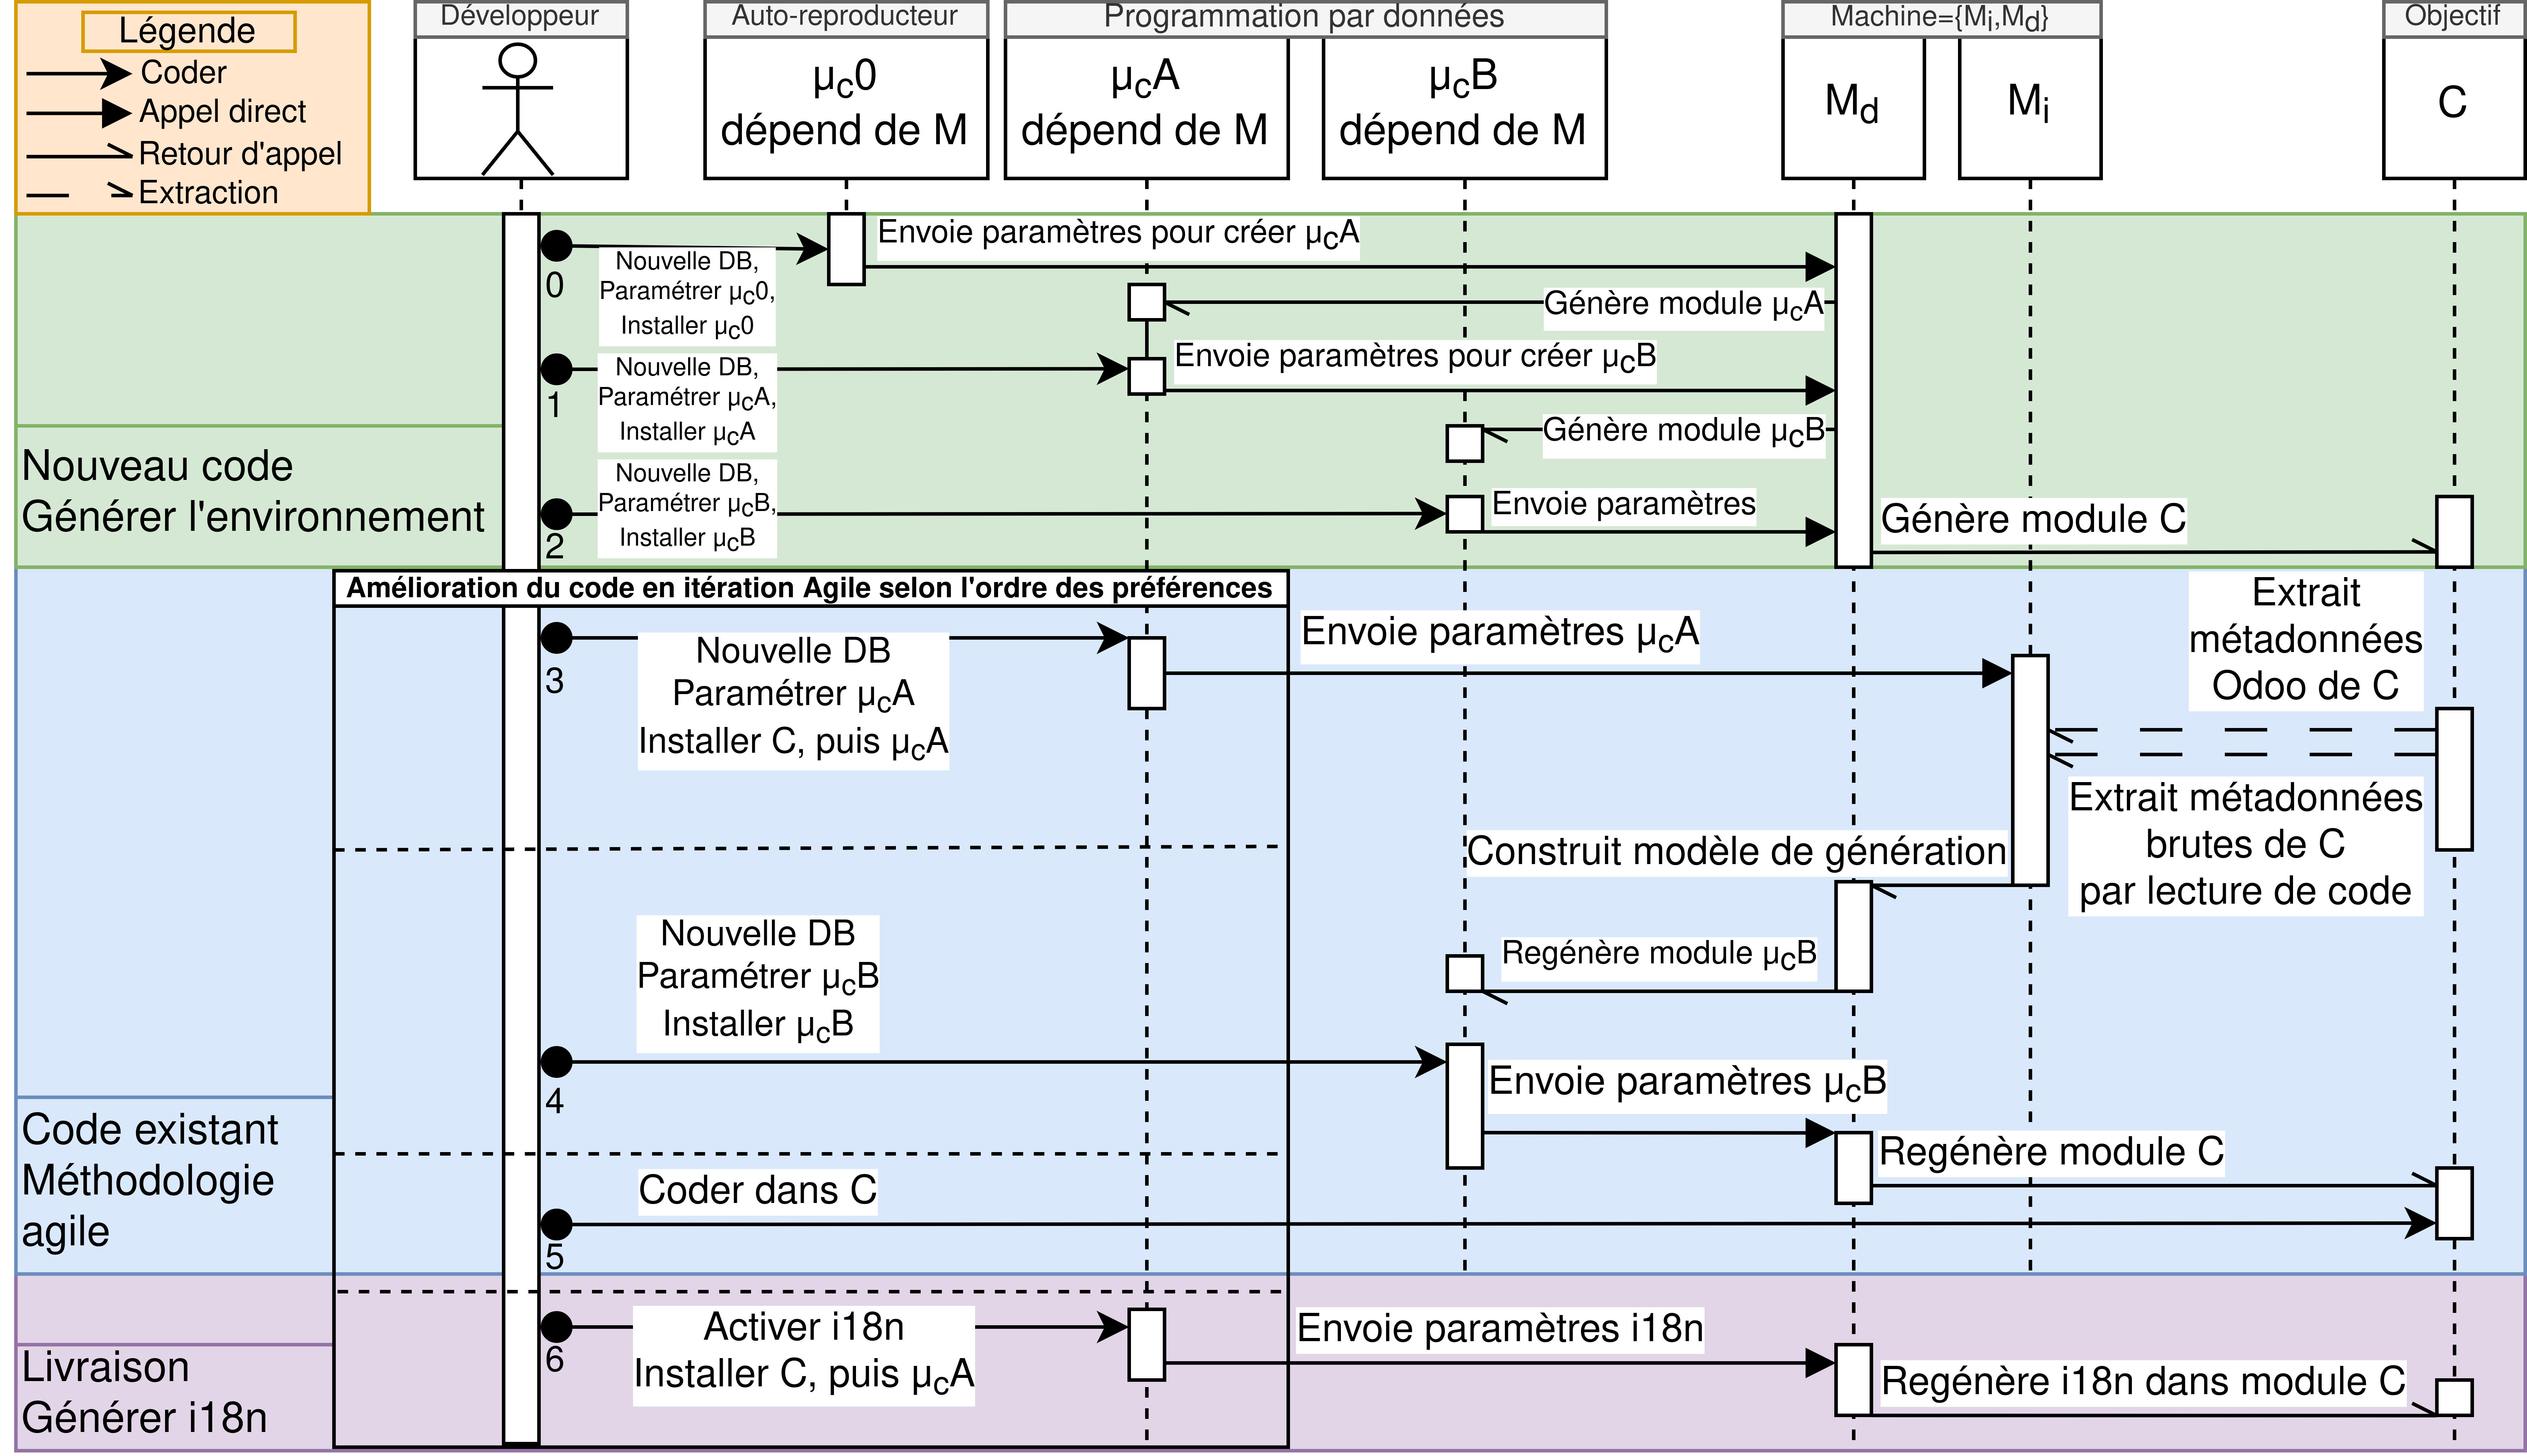
\includegraphics[width=6.535in]{images/code_generateur_erplibre_global_sequence.drawio.png}
\caption{Interaction du développeur avec le générateur de code}
\label{fig:dia_sequence_gc}
\end{figure}

Au départ d’un nouveau module code, µ$_C^0$ génère µ$_C^A$ qui génère µ$_C^B$ qui génère C. Il existe un script qui automatise un nouveau code, le développeur peut paramétrer le nom des modules et leurs emplacements. Ensuite, le développement commence en itération agile, les actions de 3 à 6 peuvent être exécutées dans l’ordre du choix du développeur.

% TODO expliquer raison/avantage de modifier soit uca, ucb ou le code directement.

Passer par l’étape 3 permet de mettre à jour l’étape 4 selon l’état du code via la rétro-ingénierie. Passer par l’étape 4 permet de mettre à jour le code selon le générateur. Il est possible de générer de nouvelles sections, comme la vue portail. Passer à l’étape 5 permet de personnaliser le code directement. Passer par l’étape 6 permet de mettre à jour le i18n de manière automatique.

La livraison sert à générer le i18n. C’est Odoo qui le génère, mais le générateur envoie les commandes, la liste des langues désirées à supporter et place les fichiers aux bons endroits dans le module. La raison pour laquelle c’est µ$_C^A$ qui doit le générer, c’est parce que le module doit être fini d’être généré et rechargé pour ensuite générer les langues, sinon ils sont corrompus par les traces de µ$_C^B$.

% TODO mettre dans discussion : Dans un contexte où l’ingénierie et la rétro-ingénierie serait parfaite, on n’aura pas besoin de mémoriser µ$_C^A$ et µ$_C^B$. Entre-temps, il y a une intervention humaine sur chacun de ces modules pour accélérer le développement. L’outil Git est utilisé pour faire des comparaisons entre les états d’itérations, seul ce qui est commité contient le bon contenu.

\subsection{Architecture}

La figure~\ref{fig:dia_architecture_automate}, elle démontre un développeur qui utilise l'interface de la machine qui opère dans le noyau de la machine.

\begin{figure}[htb]
\centering
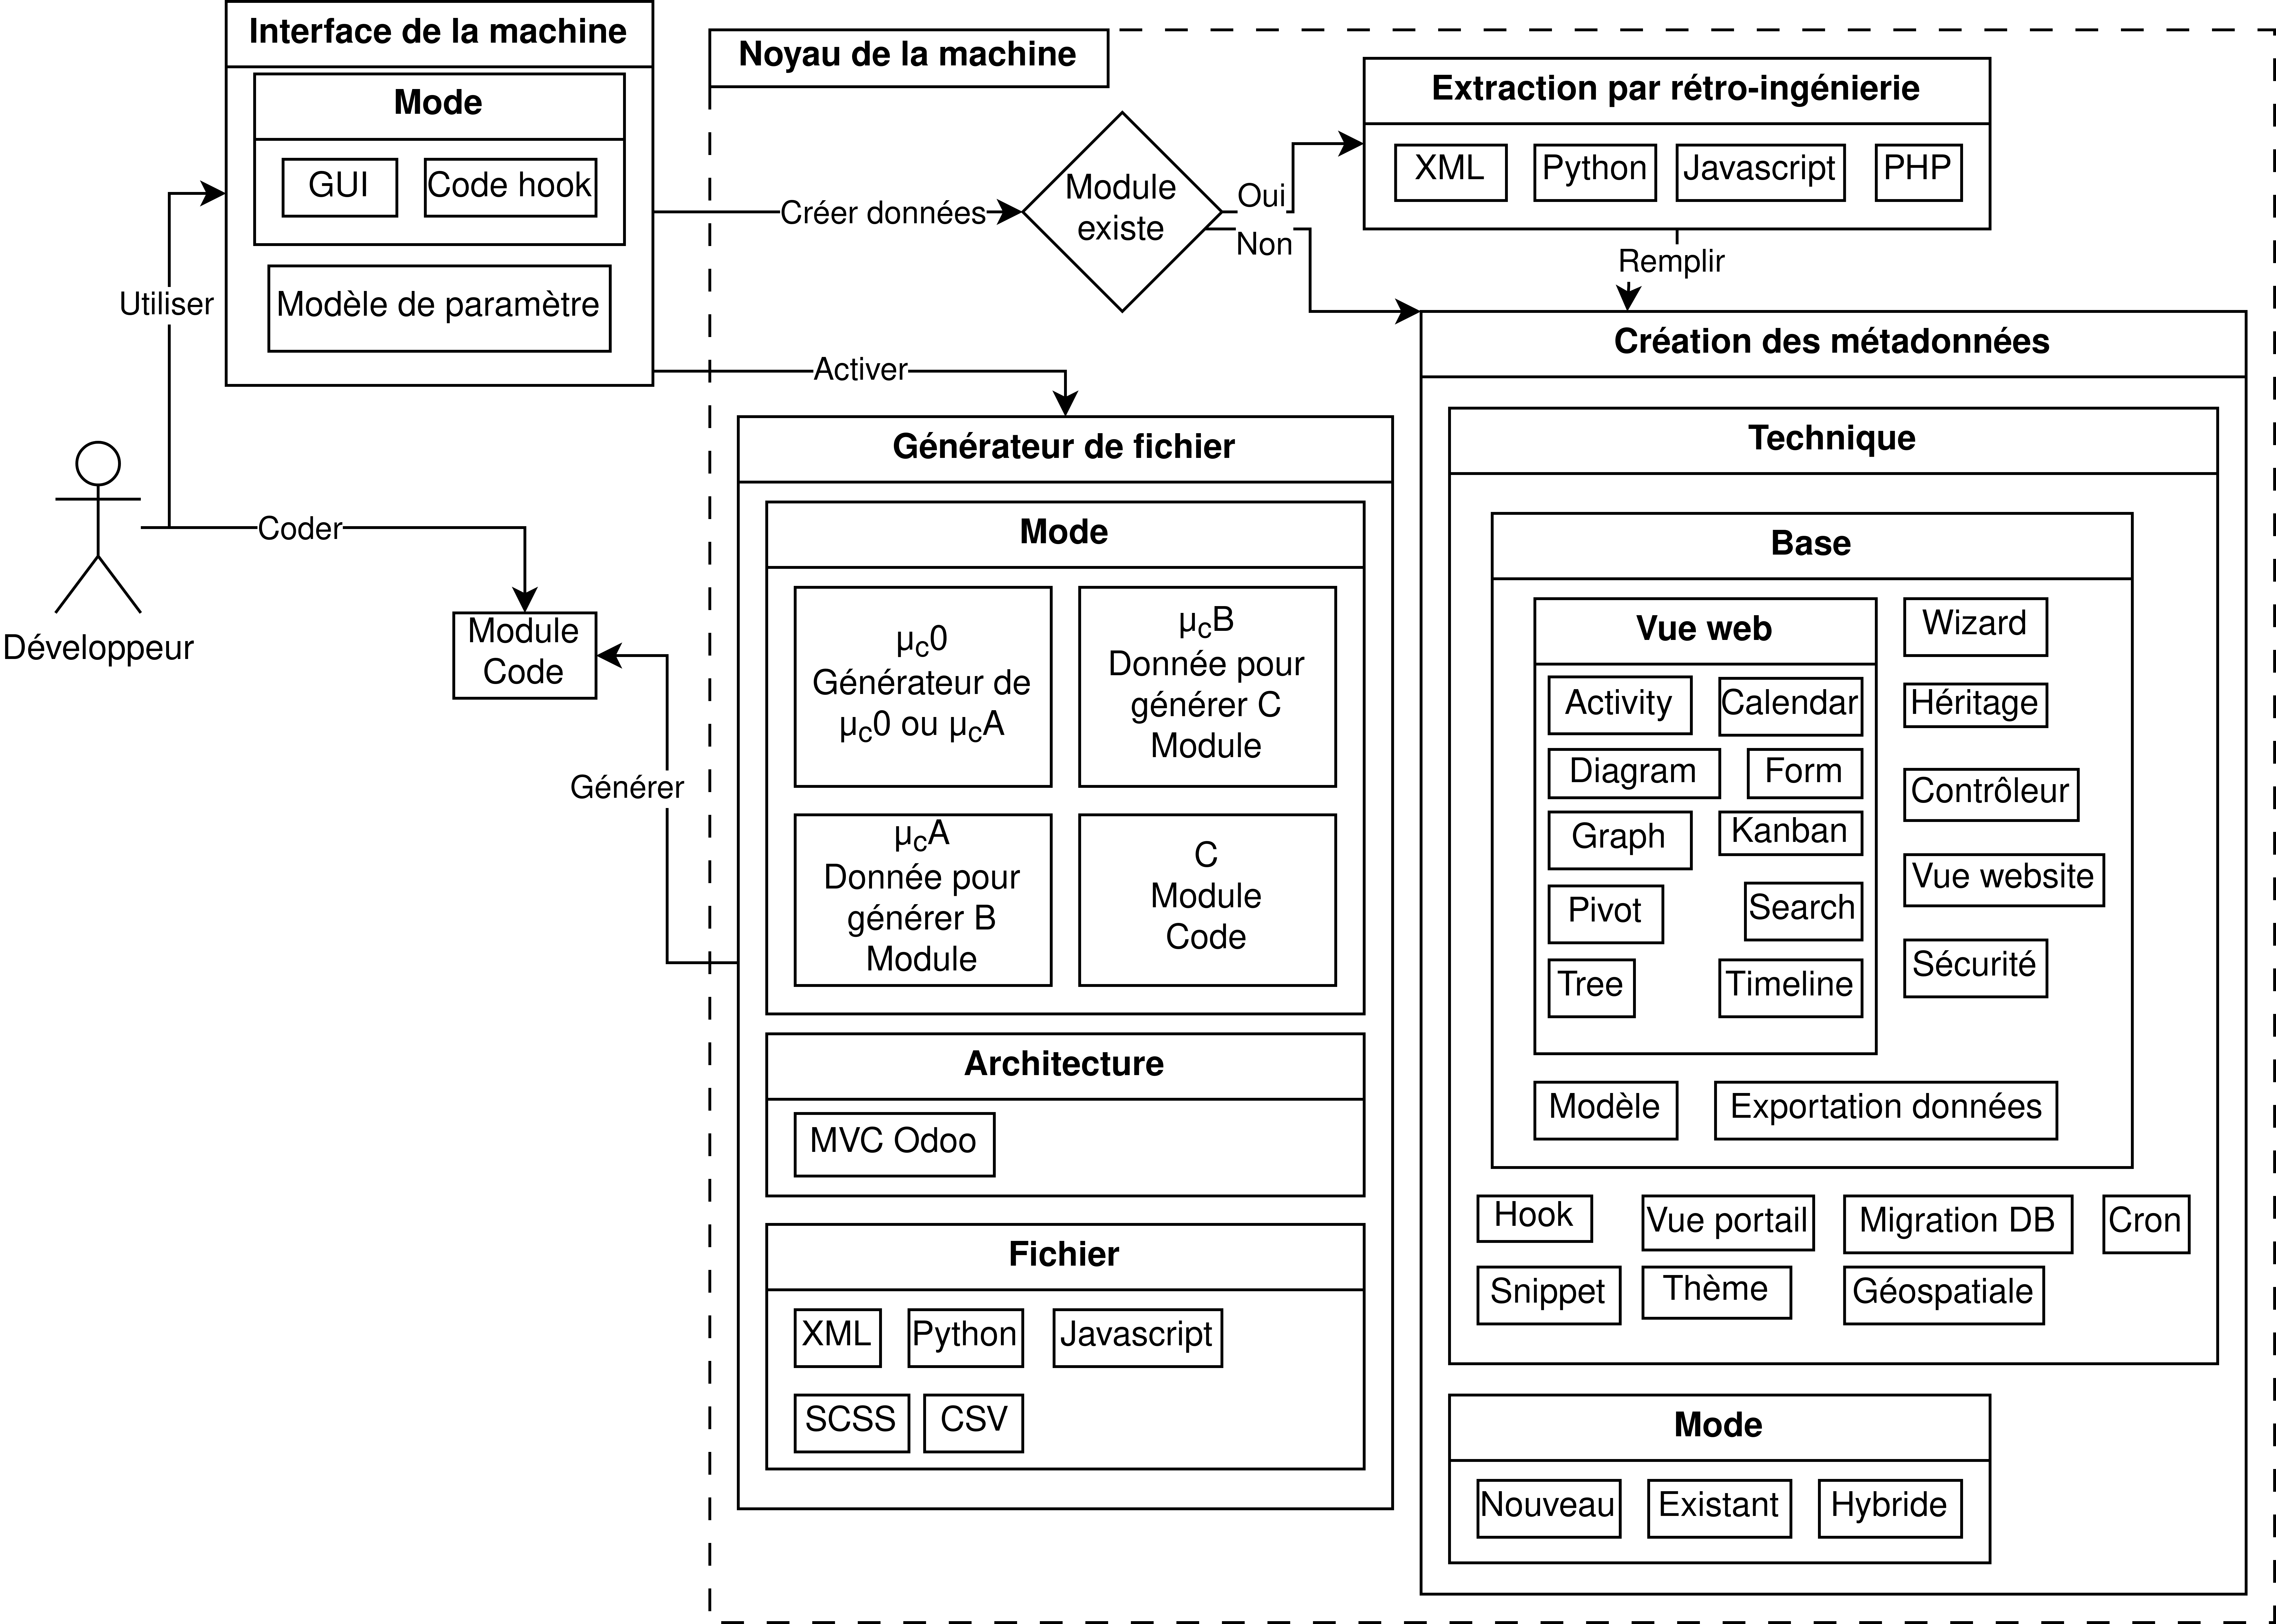
\includegraphics[width=6.535in]{images/architecture_machine.drawio.png}
\caption{Architecture de l'automate}
\label{fig:dia_architecture_automate}
\end{figure}

\begin{enumerate}
    \item L’interface machine permet à l’utilisateur de créer un modèle de données pour indiquer à la machine quelle opération effectuée avec leurs données associées. Plusieurs combinaisons, héritables, sont possibles selon les différentes techniques. De plus, c’est ici qu’on vient activer la génération de code.
    \item L’extraction par rétro-ingénierie permet de remplir le modèle de méta-données sans passer par la paramétrisation. Il extrait des informations qui ne sont pas accessibles dans le modèle de données d’Odoo sur le module.
    \item La création de méta-données se fait soit par l’utilisateur via la GUI ou le «Code Hook», il gère à la fois plusieurs techniques qui sont dans des modules. Le mode «nouveau» permet de créer de nouvelles données. Une fois qu’ils sont créés, c’est le mode «existant» qui est utilisé. Cependant le mode «hybride» permet d’écraser les données existantes en réactivant le mode «nouveau».
    \item Le générateur de fichier se fait activer par l’interface, mais il prend les méta-données pour faire sa génération selon le mode qu’il doit générer et l’architecture qu’il connaît. Il fait des liaisons entre les modèles et les vues en référence aux noms des champs de chaque modèle de données.
\end{enumerate}

Chacun de ces blocs de l’architecture est modulaire, chaque technique est héritable pour modifier le comportement et ajouter des liaisons pour permettre une génération de code au final.

La sécurité dépend du modèle. Le contrôleur dépend du modèle. La vue dépend du contrôleur et du modèle.

\subsection{Auto-générateur}

Représenté par µ$_C^0$, c’est un auto-générateur! Au moment de son installation, il génère le même code que lui-même au même endroit dans le système de fichier. Une légère modification va créer une autre entité qui sera une déviation dans l’objectif de démarrer une chaîne.

C'est le module \texttt{M} qui contient les méta-données de µ$_C^0$. Ainsi, exécuter µ$_C^0$ devient un test de fonctionnalité et c'est un succès lorsqu'il n'y a pas de différence. Cependant sa programmation est actuellement spécifique à sa génération, aucun autre module n’a besoin de cette fonctionnalité unique.

% TODO TODO calcul code unique. HOW. Regarder le nombre de ligne exécuter avec ce module VS le nombre de ligne pour un autre module simple même type -> son µ$_C^A$ avec aucun modèle et un hook.
% TODO mettre référence vers le code

% Il pourrait être plus petit, faire appel à des méthodes extérieures. De plus, il pourrait y avoir moins de paramètre, on est pris entre la faciliter de paramétrer rapidement et la gestion de la lourdeur de beaucoup de paramètres. Présentement, la machine est limitée en fonctionnalité, mais plus que ça va avancer, plus il y aura de paramètres et il en aura trop pour tous les ajouter.

L'auto-générateur est utilisé pour générer des µ$_C^A$ avec une légère modification dans les paramètres. Même s'il a la capacité de générer un µ$_C^B$, mieux vaut créer la chaîne proposé pour faire de l'amélioration continue.

\section{Résultats propres à SO-1}

\subsection{Génération par gabarit}

La génération par gabarit était déjà supportée dans la version initiale\cite{bluiksnot_repo}, de plus, il y a eu des améliorations :
